\documentclass{article}
\usepackage[utf8]{inputenc}
\usepackage[pdftex]{graphicx}
\usepackage{color, colortbl}
\usepackage{listings}


\usepackage{amsmath}
\usepackage{amssymb}

\usepackage{booktabs}

\usepackage{subcaption}

\usepackage{multirow}

\usepackage{lscape}
\usepackage{longtable}

\usepackage{pgf}

\newcolumntype{R}[1]{>{\raggedright\let\newline\\\arraybackslash\hspace{0pt}}m{#1}}

\definecolor{Gray}{gray}{0.9}

\newcommand{\vect}[1]{\boldsymbol{#1}}

\newcommand{\revised}[1]{\textcolor{blue}{#1}}

\newcommand{\acronym}{OMNI}

\usepackage{tcolorbox}

\newcounter{example}
\setcounter{example}{1}

\definecolor{exHead}{RGB}{118,103,174}
\definecolor{exMain}{RGB}{142,209,241}

\newenvironment{example}[1][]{
\begin{tcolorbox}[colback=exMain, colframe=exHead, title= \textsf{\large{\textbf{Example~\theexample. #1}}}]
\refstepcounter{example}
   \rmfamily
   \par\medskip}
{  \medskip\end{tcolorbox}}


\title{Some examples of tricky stuff in Latex}
\author{Colin Paterson }


\definecolor{prismgreen}{rgb}{0, 0.6, 0} 
\lstdefinelanguage{Prism}{ % syntax highlight via font 
        basicstyle= \ttfamily\footnotesize, % small true type font (like courier) 
        breaklines=true,
        keywords={bool,C,ceil,const,ctmc,double,dtmc,endinit,endmodule,endrewards,endsystem,F,false,
        floor,formula,G,global,I,init,int,label,max,mdp,min,module,nondeterministic,P,Pmin,Pmax,prob,
        probabilistic,R,rate,rewards,Rmin,Rmax,S,stochastic,system,true,U,X}, 
        keywordstyle={\bfseries\color{blue}}, 
        numberstyle=\tiny\color{black}, 
        morecomment=[l]{//},
        morecomment=[s]{/*}{*/},% single and multi-line 
        commentstyle=\color{prismgreen}, % dark green 
        tabsize=4, % tab treatment (going to be fixed in Prism) 
        captionpos=b, % put captions at the bottom 
        escapechar=@ % write LaTeX comments escaped by @ symbol 
} 



\begin{document}

\maketitle

\section{Introduction}

In this document I give examples of some tricky stuff that can be done in Latex that I often find myself searhing for. Note that this document is meant to be read with access to the source code.


\section{Maths equations}

This first equation requires that you have includes amsmath. Note the use f mathcal for the ``curly'' F ($\mathcal{F}$) and the use of $\backslash$\textsf{mathit} for words in maths equations.
\begin{equation}
\mathcal{F}^c((R^u_\mathit{test}, R^u_\mathit{ref}), (>)) = \begin{cases}
 {u} & \text{if}~ R^u_\mathit{test}>R^u_\mathit{ref}\\
  \emptyset & otherwise
\end{cases}
\end{equation}


Here is an example of an equation that spreads mutliple lines, note this particular example requires the amssymb package:

\begin{equation}
\begin{array}{l}
\mathit{scope}(\mathcal{L}) = \bigl\{(T_\mathit{test},T_\mathit{ref})\in \mathbb{P}\mathcal{L}\!\times\! \mathbb{P}\mathcal{L} \mid
\exists u\!\in\! \mathit{Client}\: \bullet\\
\qquad\qquad\qquad\quad \bigl(T_\mathit{test} = \{ (\mathit{id},\langle e_1, e_2, \ldots e_N \rangle)\!\in\! \mathcal{L} \mid \exists 1\leq j\leq N \bullet e_j.\mathit{user}=u\} \: \wedge \\
\qquad\qquad\qquad\qquad\qquad\quad T_\mathit{ref} = \mathcal{L}\setminus T_\mathit{test}\bigr)\bigr\}
\end{array}
\end{equation}

Next we consider multi-part equations, with each equation given the same number but a different suffix. I also show how we can make use of a new command to have vectors shown as bold. Here we include the followign command in the header. This also shows how to include code verbatim in a document, i.e. without formatting.

\begin{verbatim}
\newcommand{\vect}[1]{\boldsymbol{#1}}
\end{verbatim}

\begin{subequations}
\begin{align}
\vect{Y} &= \mathcal{M}(\vect{X}) \label{eqn:haze1} \\ \displaybreak[3]
0 &\leq \epsilon \leq p \label{eqn:haze2}\\ \displaybreak[3]
\bigwedge_{i\leq |\vect{X}|} \big( \vect{x_i} &= (1-\epsilon) x_i + \epsilon~C^f \big) \label{eqn:haze3} \\ \displaybreak[3]
\bigvee_{\substack{i<=|\vect{Y}| \\ \vect{y_i} \neq \vect{y_{real}}}} \vect{y_i} & \geq \vect{y_{real}} \label{eqn:haze4}
\end{align}
\label{eqn:haze}
\end{subequations}

\section{Some useful commands}
Sometimes it is useful to create your own commands.

A common use is to want to change the colour of text to indicate it is a revision, e.g. when  responsing to journal feedback. Here you can create a command as

\begin{verbatim}
\newcommand{\revised}[1]{\textcolor{blue}{#1}}
\end{verbatim}

and then simple \revised{change the colour by } supporting it with the new command. In this way you can later change one line and update all the colour, or search for all revisions.

Similarly you may want to use a name for the 'tool' or method you are presenting in your work, but you are unsure if you might change it later. If you create a new command like

\begin{verbatim}
    \newcommand{\acronym}{OMNI}
\end{verbatim}

Then you can include the tool name \acronym~ in your text knowing that you may change it at any time.


\section{Boxed environments}
Occasionally you might like to include a set of examples or similar in your text. I show how we can do this in the included file \textsf{exampledef.tex}. I then include this defintion in the head of the Latex document.

\begin{example}	This is the first example. But nore that I am note hard coding a number meaning that if I move this to elsewhere in the document the numbering will update. \end{example}

\begin{example}	When I add this second example the number is incremented automatically. \end{example}


\section{Figures and subfigures}

Figure~\ref{fig:CI-WebApplication} is a nice grid of equally sized graphs which makes use of the subcaption package.


\begin{figure}
	\centering
	\begin{subfigure}{0.4\textwidth}
		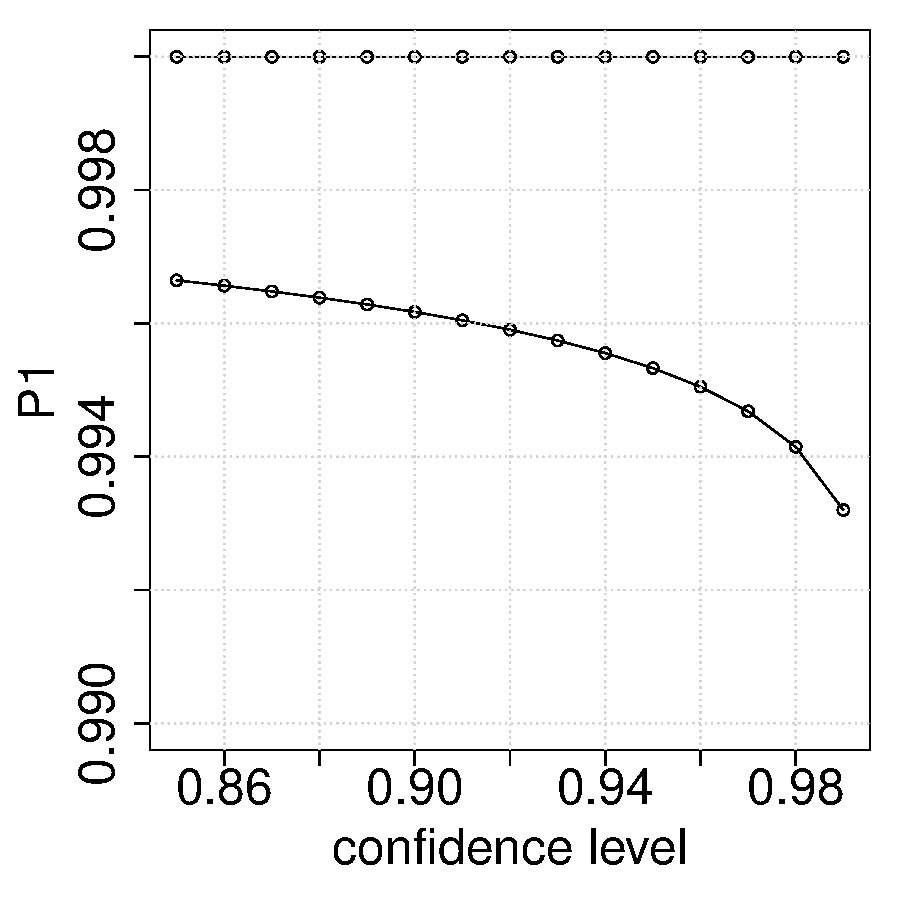
\includegraphics[width=\linewidth]{images/temp.pdf}
	\end{subfigure}
	\begin{subfigure}{0.4\textwidth}
		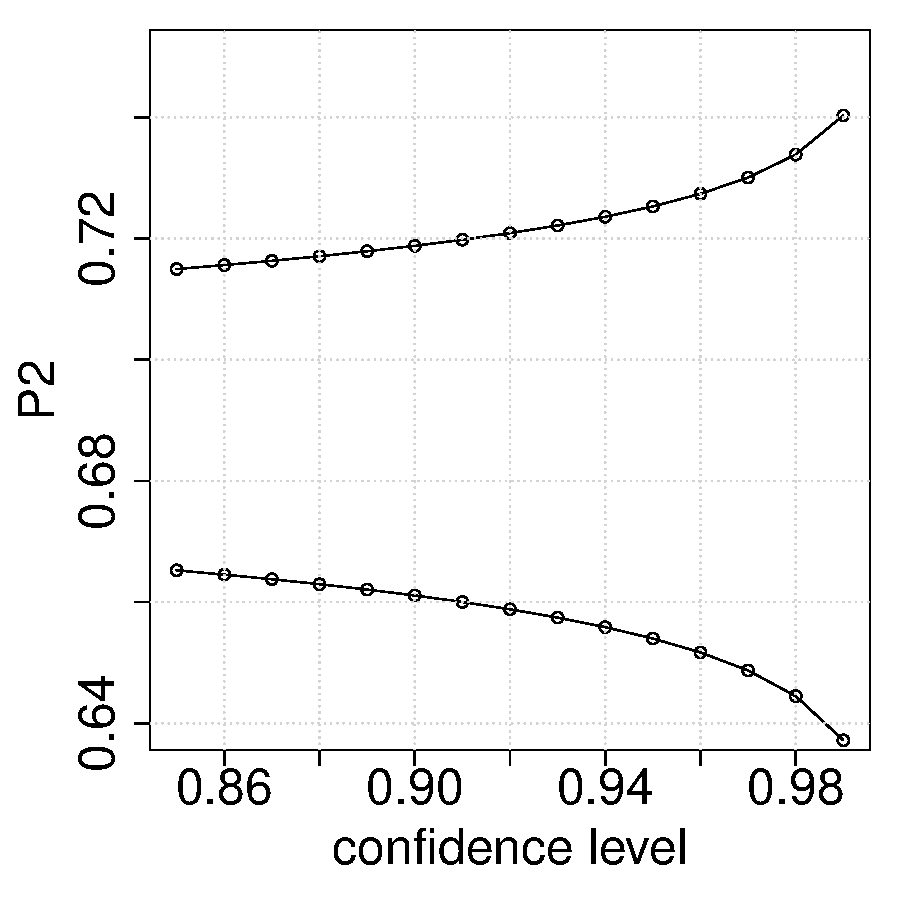
\includegraphics[width=\linewidth]{images/P2-WebApplication.pdf}
	\end{subfigure}
	\begin{subfigure}{0.4\textwidth}
		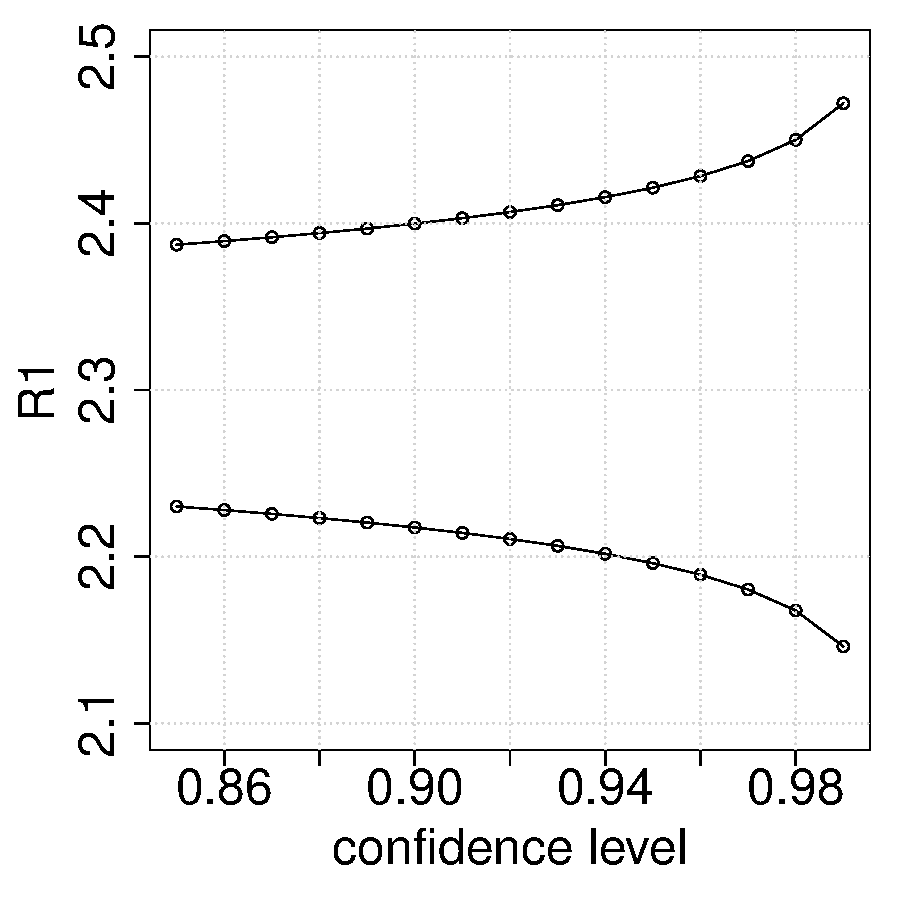
\includegraphics[width=\linewidth]{images/R1-WebApplication.pdf}
	\end{subfigure}
	\begin{subfigure}{0.4\textwidth}
		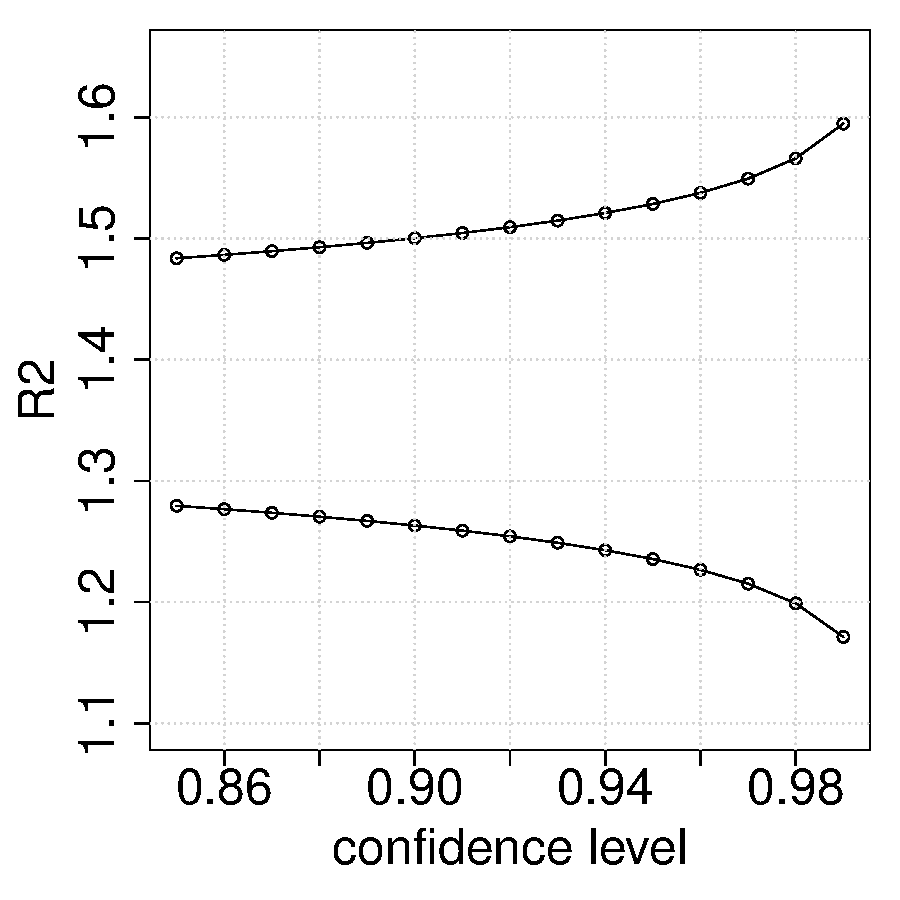
\includegraphics[width=\linewidth]{images/R2-WebApplication.pdf}
	\end{subfigure}
\caption{Confidence intervals for HTTP request process\label{fig:CI-WebApplication}}
\end{figure}


Sometimes we want to output graphs from python that have the correct fonts etc. for latex. I have uploaded three graphs generated in python called \textsf{test.png}, \textsf{test.pdf} and \textsf{test.pgf}. They are shown in Figures~\ref{fig:png},~\ref{fig:png},~\ref{fig:pgf}. Note that in the third figure I have deliberately increased the font size to demonstrate that this is the Latex font. I have also included maths in the title using standard Latex. Note that you have to start playing with margins and padding to get these perfect.

I have included the python code used to generate these graphs at the end of the document in Listing~\ref{lst:PythonCode}.


\begin{figure}
	\centering
	\begin{subfigure}{0.4\textwidth}
		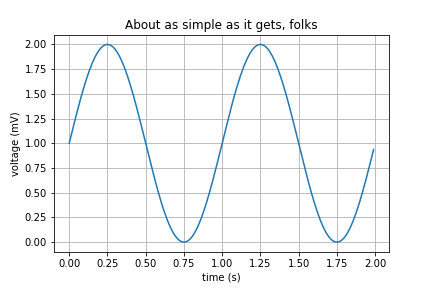
\includegraphics[width=\linewidth]{images/test.png}
        \caption{PNG image}
	\end{subfigure}
	\begin{subfigure}{0.4\textwidth}
		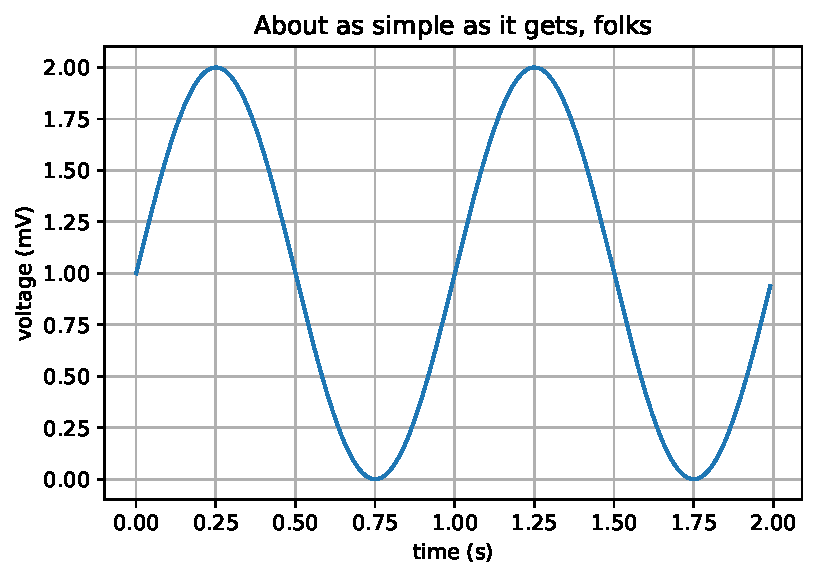
\includegraphics[width=\linewidth]{images/test.pdf}
        \caption{PDF image}
	\end{subfigure}
	\begin{subfigure}{0.4\textwidth}
		\resizebox{\textwidth}{!}{%% Creator: Matplotlib, PGF backend
%%
%% To include the figure in your LaTeX document, write
%%   \input{<filename>.pgf}
%%
%% Make sure the required packages are loaded in your preamble
%%   \usepackage{pgf}
%%
%% Figures using additional raster images can only be included by \input if
%% they are in the same directory as the main LaTeX file. For loading figures
%% from other directories you can use the `import` package
%%   \usepackage{import}
%%
%% and then include the figures with
%%   \import{<path to file>}{<filename>.pgf}
%%
%% Matplotlib used the following preamble
%%
\begingroup%
\makeatletter%
\begin{pgfpicture}%
\pgfpathrectangle{\pgfpointorigin}{\pgfqpoint{5.727774in}{4.543866in}}%
\pgfusepath{use as bounding box, clip}%
\begin{pgfscope}%
\pgfsetbuttcap%
\pgfsetmiterjoin%
\pgfsetlinewidth{0.000000pt}%
\definecolor{currentstroke}{rgb}{1.000000,1.000000,1.000000}%
\pgfsetstrokecolor{currentstroke}%
\pgfsetstrokeopacity{0.000000}%
\pgfsetdash{}{0pt}%
\pgfpathmoveto{\pgfqpoint{0.000000in}{0.000000in}}%
\pgfpathlineto{\pgfqpoint{5.727774in}{0.000000in}}%
\pgfpathlineto{\pgfqpoint{5.727774in}{4.543866in}}%
\pgfpathlineto{\pgfqpoint{0.000000in}{4.543866in}}%
\pgfpathclose%
\pgfusepath{}%
\end{pgfscope}%
\begin{pgfscope}%
\pgfsetbuttcap%
\pgfsetmiterjoin%
\definecolor{currentfill}{rgb}{1.000000,1.000000,1.000000}%
\pgfsetfillcolor{currentfill}%
\pgfsetlinewidth{0.000000pt}%
\definecolor{currentstroke}{rgb}{0.000000,0.000000,0.000000}%
\pgfsetstrokecolor{currentstroke}%
\pgfsetstrokeopacity{0.000000}%
\pgfsetdash{}{0pt}%
\pgfpathmoveto{\pgfqpoint{0.877774in}{0.805709in}}%
\pgfpathlineto{\pgfqpoint{5.527774in}{0.805709in}}%
\pgfpathlineto{\pgfqpoint{5.527774in}{3.825709in}}%
\pgfpathlineto{\pgfqpoint{0.877774in}{3.825709in}}%
\pgfpathclose%
\pgfusepath{fill}%
\end{pgfscope}%
\begin{pgfscope}%
\pgfpathrectangle{\pgfqpoint{0.877774in}{0.805709in}}{\pgfqpoint{4.650000in}{3.020000in}}%
\pgfusepath{clip}%
\pgfsetrectcap%
\pgfsetroundjoin%
\pgfsetlinewidth{0.803000pt}%
\definecolor{currentstroke}{rgb}{0.690196,0.690196,0.690196}%
\pgfsetstrokecolor{currentstroke}%
\pgfsetdash{}{0pt}%
\pgfpathmoveto{\pgfqpoint{1.089138in}{0.805709in}}%
\pgfpathlineto{\pgfqpoint{1.089138in}{3.825709in}}%
\pgfusepath{stroke}%
\end{pgfscope}%
\begin{pgfscope}%
\pgfsetbuttcap%
\pgfsetroundjoin%
\definecolor{currentfill}{rgb}{0.000000,0.000000,0.000000}%
\pgfsetfillcolor{currentfill}%
\pgfsetlinewidth{0.803000pt}%
\definecolor{currentstroke}{rgb}{0.000000,0.000000,0.000000}%
\pgfsetstrokecolor{currentstroke}%
\pgfsetdash{}{0pt}%
\pgfsys@defobject{currentmarker}{\pgfqpoint{0.000000in}{-0.048611in}}{\pgfqpoint{0.000000in}{0.000000in}}{%
\pgfpathmoveto{\pgfqpoint{0.000000in}{0.000000in}}%
\pgfpathlineto{\pgfqpoint{0.000000in}{-0.048611in}}%
\pgfusepath{stroke,fill}%
}%
\begin{pgfscope}%
\pgfsys@transformshift{1.089138in}{0.805709in}%
\pgfsys@useobject{currentmarker}{}%
\end{pgfscope}%
\end{pgfscope}%
\begin{pgfscope}%
\definecolor{textcolor}{rgb}{0.000000,0.000000,0.000000}%
\pgfsetstrokecolor{textcolor}%
\pgfsetfillcolor{textcolor}%
\pgftext[x=1.089138in,y=0.708487in,,top]{\color{textcolor}\rmfamily\fontsize{18.000000}{21.600000}\selectfont \(\displaystyle {0.0}\)}%
\end{pgfscope}%
\begin{pgfscope}%
\pgfpathrectangle{\pgfqpoint{0.877774in}{0.805709in}}{\pgfqpoint{4.650000in}{3.020000in}}%
\pgfusepath{clip}%
\pgfsetrectcap%
\pgfsetroundjoin%
\pgfsetlinewidth{0.803000pt}%
\definecolor{currentstroke}{rgb}{0.690196,0.690196,0.690196}%
\pgfsetstrokecolor{currentstroke}%
\pgfsetdash{}{0pt}%
\pgfpathmoveto{\pgfqpoint{2.151266in}{0.805709in}}%
\pgfpathlineto{\pgfqpoint{2.151266in}{3.825709in}}%
\pgfusepath{stroke}%
\end{pgfscope}%
\begin{pgfscope}%
\pgfsetbuttcap%
\pgfsetroundjoin%
\definecolor{currentfill}{rgb}{0.000000,0.000000,0.000000}%
\pgfsetfillcolor{currentfill}%
\pgfsetlinewidth{0.803000pt}%
\definecolor{currentstroke}{rgb}{0.000000,0.000000,0.000000}%
\pgfsetstrokecolor{currentstroke}%
\pgfsetdash{}{0pt}%
\pgfsys@defobject{currentmarker}{\pgfqpoint{0.000000in}{-0.048611in}}{\pgfqpoint{0.000000in}{0.000000in}}{%
\pgfpathmoveto{\pgfqpoint{0.000000in}{0.000000in}}%
\pgfpathlineto{\pgfqpoint{0.000000in}{-0.048611in}}%
\pgfusepath{stroke,fill}%
}%
\begin{pgfscope}%
\pgfsys@transformshift{2.151266in}{0.805709in}%
\pgfsys@useobject{currentmarker}{}%
\end{pgfscope}%
\end{pgfscope}%
\begin{pgfscope}%
\definecolor{textcolor}{rgb}{0.000000,0.000000,0.000000}%
\pgfsetstrokecolor{textcolor}%
\pgfsetfillcolor{textcolor}%
\pgftext[x=2.151266in,y=0.708487in,,top]{\color{textcolor}\rmfamily\fontsize{18.000000}{21.600000}\selectfont \(\displaystyle {0.5}\)}%
\end{pgfscope}%
\begin{pgfscope}%
\pgfpathrectangle{\pgfqpoint{0.877774in}{0.805709in}}{\pgfqpoint{4.650000in}{3.020000in}}%
\pgfusepath{clip}%
\pgfsetrectcap%
\pgfsetroundjoin%
\pgfsetlinewidth{0.803000pt}%
\definecolor{currentstroke}{rgb}{0.690196,0.690196,0.690196}%
\pgfsetstrokecolor{currentstroke}%
\pgfsetdash{}{0pt}%
\pgfpathmoveto{\pgfqpoint{3.213395in}{0.805709in}}%
\pgfpathlineto{\pgfqpoint{3.213395in}{3.825709in}}%
\pgfusepath{stroke}%
\end{pgfscope}%
\begin{pgfscope}%
\pgfsetbuttcap%
\pgfsetroundjoin%
\definecolor{currentfill}{rgb}{0.000000,0.000000,0.000000}%
\pgfsetfillcolor{currentfill}%
\pgfsetlinewidth{0.803000pt}%
\definecolor{currentstroke}{rgb}{0.000000,0.000000,0.000000}%
\pgfsetstrokecolor{currentstroke}%
\pgfsetdash{}{0pt}%
\pgfsys@defobject{currentmarker}{\pgfqpoint{0.000000in}{-0.048611in}}{\pgfqpoint{0.000000in}{0.000000in}}{%
\pgfpathmoveto{\pgfqpoint{0.000000in}{0.000000in}}%
\pgfpathlineto{\pgfqpoint{0.000000in}{-0.048611in}}%
\pgfusepath{stroke,fill}%
}%
\begin{pgfscope}%
\pgfsys@transformshift{3.213395in}{0.805709in}%
\pgfsys@useobject{currentmarker}{}%
\end{pgfscope}%
\end{pgfscope}%
\begin{pgfscope}%
\definecolor{textcolor}{rgb}{0.000000,0.000000,0.000000}%
\pgfsetstrokecolor{textcolor}%
\pgfsetfillcolor{textcolor}%
\pgftext[x=3.213395in,y=0.708487in,,top]{\color{textcolor}\rmfamily\fontsize{18.000000}{21.600000}\selectfont \(\displaystyle {1.0}\)}%
\end{pgfscope}%
\begin{pgfscope}%
\pgfpathrectangle{\pgfqpoint{0.877774in}{0.805709in}}{\pgfqpoint{4.650000in}{3.020000in}}%
\pgfusepath{clip}%
\pgfsetrectcap%
\pgfsetroundjoin%
\pgfsetlinewidth{0.803000pt}%
\definecolor{currentstroke}{rgb}{0.690196,0.690196,0.690196}%
\pgfsetstrokecolor{currentstroke}%
\pgfsetdash{}{0pt}%
\pgfpathmoveto{\pgfqpoint{4.275524in}{0.805709in}}%
\pgfpathlineto{\pgfqpoint{4.275524in}{3.825709in}}%
\pgfusepath{stroke}%
\end{pgfscope}%
\begin{pgfscope}%
\pgfsetbuttcap%
\pgfsetroundjoin%
\definecolor{currentfill}{rgb}{0.000000,0.000000,0.000000}%
\pgfsetfillcolor{currentfill}%
\pgfsetlinewidth{0.803000pt}%
\definecolor{currentstroke}{rgb}{0.000000,0.000000,0.000000}%
\pgfsetstrokecolor{currentstroke}%
\pgfsetdash{}{0pt}%
\pgfsys@defobject{currentmarker}{\pgfqpoint{0.000000in}{-0.048611in}}{\pgfqpoint{0.000000in}{0.000000in}}{%
\pgfpathmoveto{\pgfqpoint{0.000000in}{0.000000in}}%
\pgfpathlineto{\pgfqpoint{0.000000in}{-0.048611in}}%
\pgfusepath{stroke,fill}%
}%
\begin{pgfscope}%
\pgfsys@transformshift{4.275524in}{0.805709in}%
\pgfsys@useobject{currentmarker}{}%
\end{pgfscope}%
\end{pgfscope}%
\begin{pgfscope}%
\definecolor{textcolor}{rgb}{0.000000,0.000000,0.000000}%
\pgfsetstrokecolor{textcolor}%
\pgfsetfillcolor{textcolor}%
\pgftext[x=4.275524in,y=0.708487in,,top]{\color{textcolor}\rmfamily\fontsize{18.000000}{21.600000}\selectfont \(\displaystyle {1.5}\)}%
\end{pgfscope}%
\begin{pgfscope}%
\pgfpathrectangle{\pgfqpoint{0.877774in}{0.805709in}}{\pgfqpoint{4.650000in}{3.020000in}}%
\pgfusepath{clip}%
\pgfsetrectcap%
\pgfsetroundjoin%
\pgfsetlinewidth{0.803000pt}%
\definecolor{currentstroke}{rgb}{0.690196,0.690196,0.690196}%
\pgfsetstrokecolor{currentstroke}%
\pgfsetdash{}{0pt}%
\pgfpathmoveto{\pgfqpoint{5.337653in}{0.805709in}}%
\pgfpathlineto{\pgfqpoint{5.337653in}{3.825709in}}%
\pgfusepath{stroke}%
\end{pgfscope}%
\begin{pgfscope}%
\pgfsetbuttcap%
\pgfsetroundjoin%
\definecolor{currentfill}{rgb}{0.000000,0.000000,0.000000}%
\pgfsetfillcolor{currentfill}%
\pgfsetlinewidth{0.803000pt}%
\definecolor{currentstroke}{rgb}{0.000000,0.000000,0.000000}%
\pgfsetstrokecolor{currentstroke}%
\pgfsetdash{}{0pt}%
\pgfsys@defobject{currentmarker}{\pgfqpoint{0.000000in}{-0.048611in}}{\pgfqpoint{0.000000in}{0.000000in}}{%
\pgfpathmoveto{\pgfqpoint{0.000000in}{0.000000in}}%
\pgfpathlineto{\pgfqpoint{0.000000in}{-0.048611in}}%
\pgfusepath{stroke,fill}%
}%
\begin{pgfscope}%
\pgfsys@transformshift{5.337653in}{0.805709in}%
\pgfsys@useobject{currentmarker}{}%
\end{pgfscope}%
\end{pgfscope}%
\begin{pgfscope}%
\definecolor{textcolor}{rgb}{0.000000,0.000000,0.000000}%
\pgfsetstrokecolor{textcolor}%
\pgfsetfillcolor{textcolor}%
\pgftext[x=5.337653in,y=0.708487in,,top]{\color{textcolor}\rmfamily\fontsize{18.000000}{21.600000}\selectfont \(\displaystyle {2.0}\)}%
\end{pgfscope}%
\begin{pgfscope}%
\definecolor{textcolor}{rgb}{0.000000,0.000000,0.000000}%
\pgfsetstrokecolor{textcolor}%
\pgfsetfillcolor{textcolor}%
\pgftext[x=3.202774in,y=0.439583in,,top]{\color{textcolor}\rmfamily\fontsize{18.000000}{21.600000}\selectfont time (s)}%
\end{pgfscope}%
\begin{pgfscope}%
\pgfpathrectangle{\pgfqpoint{0.877774in}{0.805709in}}{\pgfqpoint{4.650000in}{3.020000in}}%
\pgfusepath{clip}%
\pgfsetrectcap%
\pgfsetroundjoin%
\pgfsetlinewidth{0.803000pt}%
\definecolor{currentstroke}{rgb}{0.690196,0.690196,0.690196}%
\pgfsetstrokecolor{currentstroke}%
\pgfsetdash{}{0pt}%
\pgfpathmoveto{\pgfqpoint{0.877774in}{0.942982in}}%
\pgfpathlineto{\pgfqpoint{5.527774in}{0.942982in}}%
\pgfusepath{stroke}%
\end{pgfscope}%
\begin{pgfscope}%
\pgfsetbuttcap%
\pgfsetroundjoin%
\definecolor{currentfill}{rgb}{0.000000,0.000000,0.000000}%
\pgfsetfillcolor{currentfill}%
\pgfsetlinewidth{0.803000pt}%
\definecolor{currentstroke}{rgb}{0.000000,0.000000,0.000000}%
\pgfsetstrokecolor{currentstroke}%
\pgfsetdash{}{0pt}%
\pgfsys@defobject{currentmarker}{\pgfqpoint{-0.048611in}{0.000000in}}{\pgfqpoint{-0.000000in}{0.000000in}}{%
\pgfpathmoveto{\pgfqpoint{-0.000000in}{0.000000in}}%
\pgfpathlineto{\pgfqpoint{-0.048611in}{0.000000in}}%
\pgfusepath{stroke,fill}%
}%
\begin{pgfscope}%
\pgfsys@transformshift{0.877774in}{0.942982in}%
\pgfsys@useobject{currentmarker}{}%
\end{pgfscope}%
\end{pgfscope}%
\begin{pgfscope}%
\definecolor{textcolor}{rgb}{0.000000,0.000000,0.000000}%
\pgfsetstrokecolor{textcolor}%
\pgfsetfillcolor{textcolor}%
\pgftext[x=0.495138in, y=0.859649in, left, base]{\color{textcolor}\rmfamily\fontsize{18.000000}{21.600000}\selectfont \(\displaystyle {0.0}\)}%
\end{pgfscope}%
\begin{pgfscope}%
\pgfpathrectangle{\pgfqpoint{0.877774in}{0.805709in}}{\pgfqpoint{4.650000in}{3.020000in}}%
\pgfusepath{clip}%
\pgfsetrectcap%
\pgfsetroundjoin%
\pgfsetlinewidth{0.803000pt}%
\definecolor{currentstroke}{rgb}{0.690196,0.690196,0.690196}%
\pgfsetstrokecolor{currentstroke}%
\pgfsetdash{}{0pt}%
\pgfpathmoveto{\pgfqpoint{0.877774in}{1.629346in}}%
\pgfpathlineto{\pgfqpoint{5.527774in}{1.629346in}}%
\pgfusepath{stroke}%
\end{pgfscope}%
\begin{pgfscope}%
\pgfsetbuttcap%
\pgfsetroundjoin%
\definecolor{currentfill}{rgb}{0.000000,0.000000,0.000000}%
\pgfsetfillcolor{currentfill}%
\pgfsetlinewidth{0.803000pt}%
\definecolor{currentstroke}{rgb}{0.000000,0.000000,0.000000}%
\pgfsetstrokecolor{currentstroke}%
\pgfsetdash{}{0pt}%
\pgfsys@defobject{currentmarker}{\pgfqpoint{-0.048611in}{0.000000in}}{\pgfqpoint{-0.000000in}{0.000000in}}{%
\pgfpathmoveto{\pgfqpoint{-0.000000in}{0.000000in}}%
\pgfpathlineto{\pgfqpoint{-0.048611in}{0.000000in}}%
\pgfusepath{stroke,fill}%
}%
\begin{pgfscope}%
\pgfsys@transformshift{0.877774in}{1.629346in}%
\pgfsys@useobject{currentmarker}{}%
\end{pgfscope}%
\end{pgfscope}%
\begin{pgfscope}%
\definecolor{textcolor}{rgb}{0.000000,0.000000,0.000000}%
\pgfsetstrokecolor{textcolor}%
\pgfsetfillcolor{textcolor}%
\pgftext[x=0.495138in, y=1.546012in, left, base]{\color{textcolor}\rmfamily\fontsize{18.000000}{21.600000}\selectfont \(\displaystyle {0.5}\)}%
\end{pgfscope}%
\begin{pgfscope}%
\pgfpathrectangle{\pgfqpoint{0.877774in}{0.805709in}}{\pgfqpoint{4.650000in}{3.020000in}}%
\pgfusepath{clip}%
\pgfsetrectcap%
\pgfsetroundjoin%
\pgfsetlinewidth{0.803000pt}%
\definecolor{currentstroke}{rgb}{0.690196,0.690196,0.690196}%
\pgfsetstrokecolor{currentstroke}%
\pgfsetdash{}{0pt}%
\pgfpathmoveto{\pgfqpoint{0.877774in}{2.315709in}}%
\pgfpathlineto{\pgfqpoint{5.527774in}{2.315709in}}%
\pgfusepath{stroke}%
\end{pgfscope}%
\begin{pgfscope}%
\pgfsetbuttcap%
\pgfsetroundjoin%
\definecolor{currentfill}{rgb}{0.000000,0.000000,0.000000}%
\pgfsetfillcolor{currentfill}%
\pgfsetlinewidth{0.803000pt}%
\definecolor{currentstroke}{rgb}{0.000000,0.000000,0.000000}%
\pgfsetstrokecolor{currentstroke}%
\pgfsetdash{}{0pt}%
\pgfsys@defobject{currentmarker}{\pgfqpoint{-0.048611in}{0.000000in}}{\pgfqpoint{-0.000000in}{0.000000in}}{%
\pgfpathmoveto{\pgfqpoint{-0.000000in}{0.000000in}}%
\pgfpathlineto{\pgfqpoint{-0.048611in}{0.000000in}}%
\pgfusepath{stroke,fill}%
}%
\begin{pgfscope}%
\pgfsys@transformshift{0.877774in}{2.315709in}%
\pgfsys@useobject{currentmarker}{}%
\end{pgfscope}%
\end{pgfscope}%
\begin{pgfscope}%
\definecolor{textcolor}{rgb}{0.000000,0.000000,0.000000}%
\pgfsetstrokecolor{textcolor}%
\pgfsetfillcolor{textcolor}%
\pgftext[x=0.495138in, y=2.232376in, left, base]{\color{textcolor}\rmfamily\fontsize{18.000000}{21.600000}\selectfont \(\displaystyle {1.0}\)}%
\end{pgfscope}%
\begin{pgfscope}%
\pgfpathrectangle{\pgfqpoint{0.877774in}{0.805709in}}{\pgfqpoint{4.650000in}{3.020000in}}%
\pgfusepath{clip}%
\pgfsetrectcap%
\pgfsetroundjoin%
\pgfsetlinewidth{0.803000pt}%
\definecolor{currentstroke}{rgb}{0.690196,0.690196,0.690196}%
\pgfsetstrokecolor{currentstroke}%
\pgfsetdash{}{0pt}%
\pgfpathmoveto{\pgfqpoint{0.877774in}{3.002073in}}%
\pgfpathlineto{\pgfqpoint{5.527774in}{3.002073in}}%
\pgfusepath{stroke}%
\end{pgfscope}%
\begin{pgfscope}%
\pgfsetbuttcap%
\pgfsetroundjoin%
\definecolor{currentfill}{rgb}{0.000000,0.000000,0.000000}%
\pgfsetfillcolor{currentfill}%
\pgfsetlinewidth{0.803000pt}%
\definecolor{currentstroke}{rgb}{0.000000,0.000000,0.000000}%
\pgfsetstrokecolor{currentstroke}%
\pgfsetdash{}{0pt}%
\pgfsys@defobject{currentmarker}{\pgfqpoint{-0.048611in}{0.000000in}}{\pgfqpoint{-0.000000in}{0.000000in}}{%
\pgfpathmoveto{\pgfqpoint{-0.000000in}{0.000000in}}%
\pgfpathlineto{\pgfqpoint{-0.048611in}{0.000000in}}%
\pgfusepath{stroke,fill}%
}%
\begin{pgfscope}%
\pgfsys@transformshift{0.877774in}{3.002073in}%
\pgfsys@useobject{currentmarker}{}%
\end{pgfscope}%
\end{pgfscope}%
\begin{pgfscope}%
\definecolor{textcolor}{rgb}{0.000000,0.000000,0.000000}%
\pgfsetstrokecolor{textcolor}%
\pgfsetfillcolor{textcolor}%
\pgftext[x=0.495138in, y=2.918740in, left, base]{\color{textcolor}\rmfamily\fontsize{18.000000}{21.600000}\selectfont \(\displaystyle {1.5}\)}%
\end{pgfscope}%
\begin{pgfscope}%
\pgfpathrectangle{\pgfqpoint{0.877774in}{0.805709in}}{\pgfqpoint{4.650000in}{3.020000in}}%
\pgfusepath{clip}%
\pgfsetrectcap%
\pgfsetroundjoin%
\pgfsetlinewidth{0.803000pt}%
\definecolor{currentstroke}{rgb}{0.690196,0.690196,0.690196}%
\pgfsetstrokecolor{currentstroke}%
\pgfsetdash{}{0pt}%
\pgfpathmoveto{\pgfqpoint{0.877774in}{3.688437in}}%
\pgfpathlineto{\pgfqpoint{5.527774in}{3.688437in}}%
\pgfusepath{stroke}%
\end{pgfscope}%
\begin{pgfscope}%
\pgfsetbuttcap%
\pgfsetroundjoin%
\definecolor{currentfill}{rgb}{0.000000,0.000000,0.000000}%
\pgfsetfillcolor{currentfill}%
\pgfsetlinewidth{0.803000pt}%
\definecolor{currentstroke}{rgb}{0.000000,0.000000,0.000000}%
\pgfsetstrokecolor{currentstroke}%
\pgfsetdash{}{0pt}%
\pgfsys@defobject{currentmarker}{\pgfqpoint{-0.048611in}{0.000000in}}{\pgfqpoint{-0.000000in}{0.000000in}}{%
\pgfpathmoveto{\pgfqpoint{-0.000000in}{0.000000in}}%
\pgfpathlineto{\pgfqpoint{-0.048611in}{0.000000in}}%
\pgfusepath{stroke,fill}%
}%
\begin{pgfscope}%
\pgfsys@transformshift{0.877774in}{3.688437in}%
\pgfsys@useobject{currentmarker}{}%
\end{pgfscope}%
\end{pgfscope}%
\begin{pgfscope}%
\definecolor{textcolor}{rgb}{0.000000,0.000000,0.000000}%
\pgfsetstrokecolor{textcolor}%
\pgfsetfillcolor{textcolor}%
\pgftext[x=0.495138in, y=3.605103in, left, base]{\color{textcolor}\rmfamily\fontsize{18.000000}{21.600000}\selectfont \(\displaystyle {2.0}\)}%
\end{pgfscope}%
\begin{pgfscope}%
\definecolor{textcolor}{rgb}{0.000000,0.000000,0.000000}%
\pgfsetstrokecolor{textcolor}%
\pgfsetfillcolor{textcolor}%
\pgftext[x=0.439583in,y=2.315709in,,bottom,rotate=90.000000]{\color{textcolor}\rmfamily\fontsize{18.000000}{21.600000}\selectfont voltage (mV)}%
\end{pgfscope}%
\begin{pgfscope}%
\pgfpathrectangle{\pgfqpoint{0.877774in}{0.805709in}}{\pgfqpoint{4.650000in}{3.020000in}}%
\pgfusepath{clip}%
\pgfsetrectcap%
\pgfsetroundjoin%
\pgfsetlinewidth{1.505625pt}%
\definecolor{currentstroke}{rgb}{0.121569,0.466667,0.705882}%
\pgfsetstrokecolor{currentstroke}%
\pgfsetdash{}{0pt}%
\pgfpathmoveto{\pgfqpoint{1.089138in}{2.315709in}}%
\pgfpathlineto{\pgfqpoint{1.174108in}{2.657093in}}%
\pgfpathlineto{\pgfqpoint{1.237836in}{2.900188in}}%
\pgfpathlineto{\pgfqpoint{1.280321in}{3.051253in}}%
\pgfpathlineto{\pgfqpoint{1.322806in}{3.190719in}}%
\pgfpathlineto{\pgfqpoint{1.365291in}{3.316384in}}%
\pgfpathlineto{\pgfqpoint{1.407776in}{3.426269in}}%
\pgfpathlineto{\pgfqpoint{1.429019in}{3.474741in}}%
\pgfpathlineto{\pgfqpoint{1.450261in}{3.518639in}}%
\pgfpathlineto{\pgfqpoint{1.471504in}{3.557790in}}%
\pgfpathlineto{\pgfqpoint{1.492747in}{3.592039in}}%
\pgfpathlineto{\pgfqpoint{1.513989in}{3.621251in}}%
\pgfpathlineto{\pgfqpoint{1.535232in}{3.645310in}}%
\pgfpathlineto{\pgfqpoint{1.556474in}{3.664122in}}%
\pgfpathlineto{\pgfqpoint{1.577717in}{3.677612in}}%
\pgfpathlineto{\pgfqpoint{1.598960in}{3.685728in}}%
\pgfpathlineto{\pgfqpoint{1.620202in}{3.688437in}}%
\pgfpathlineto{\pgfqpoint{1.641445in}{3.685728in}}%
\pgfpathlineto{\pgfqpoint{1.662687in}{3.677612in}}%
\pgfpathlineto{\pgfqpoint{1.683930in}{3.664122in}}%
\pgfpathlineto{\pgfqpoint{1.705172in}{3.645310in}}%
\pgfpathlineto{\pgfqpoint{1.726415in}{3.621251in}}%
\pgfpathlineto{\pgfqpoint{1.747658in}{3.592039in}}%
\pgfpathlineto{\pgfqpoint{1.768900in}{3.557790in}}%
\pgfpathlineto{\pgfqpoint{1.790143in}{3.518639in}}%
\pgfpathlineto{\pgfqpoint{1.811385in}{3.474741in}}%
\pgfpathlineto{\pgfqpoint{1.832628in}{3.426269in}}%
\pgfpathlineto{\pgfqpoint{1.853870in}{3.373414in}}%
\pgfpathlineto{\pgfqpoint{1.896356in}{3.255406in}}%
\pgfpathlineto{\pgfqpoint{1.938841in}{3.122578in}}%
\pgfpathlineto{\pgfqpoint{1.981326in}{2.977026in}}%
\pgfpathlineto{\pgfqpoint{2.023811in}{2.821044in}}%
\pgfpathlineto{\pgfqpoint{2.087539in}{2.572933in}}%
\pgfpathlineto{\pgfqpoint{2.278722in}{1.810375in}}%
\pgfpathlineto{\pgfqpoint{2.321207in}{1.654393in}}%
\pgfpathlineto{\pgfqpoint{2.363692in}{1.508840in}}%
\pgfpathlineto{\pgfqpoint{2.406177in}{1.376013in}}%
\pgfpathlineto{\pgfqpoint{2.448663in}{1.258005in}}%
\pgfpathlineto{\pgfqpoint{2.469905in}{1.205150in}}%
\pgfpathlineto{\pgfqpoint{2.491148in}{1.156677in}}%
\pgfpathlineto{\pgfqpoint{2.512390in}{1.112779in}}%
\pgfpathlineto{\pgfqpoint{2.533633in}{1.073629in}}%
\pgfpathlineto{\pgfqpoint{2.554875in}{1.039380in}}%
\pgfpathlineto{\pgfqpoint{2.576118in}{1.010168in}}%
\pgfpathlineto{\pgfqpoint{2.597361in}{0.986109in}}%
\pgfpathlineto{\pgfqpoint{2.618603in}{0.967297in}}%
\pgfpathlineto{\pgfqpoint{2.639846in}{0.953806in}}%
\pgfpathlineto{\pgfqpoint{2.661088in}{0.945691in}}%
\pgfpathlineto{\pgfqpoint{2.682331in}{0.942982in}}%
\pgfpathlineto{\pgfqpoint{2.703573in}{0.945691in}}%
\pgfpathlineto{\pgfqpoint{2.724816in}{0.953806in}}%
\pgfpathlineto{\pgfqpoint{2.746059in}{0.967297in}}%
\pgfpathlineto{\pgfqpoint{2.767301in}{0.986109in}}%
\pgfpathlineto{\pgfqpoint{2.788544in}{1.010168in}}%
\pgfpathlineto{\pgfqpoint{2.809786in}{1.039380in}}%
\pgfpathlineto{\pgfqpoint{2.831029in}{1.073629in}}%
\pgfpathlineto{\pgfqpoint{2.852272in}{1.112779in}}%
\pgfpathlineto{\pgfqpoint{2.873514in}{1.156677in}}%
\pgfpathlineto{\pgfqpoint{2.894757in}{1.205150in}}%
\pgfpathlineto{\pgfqpoint{2.915999in}{1.258005in}}%
\pgfpathlineto{\pgfqpoint{2.958484in}{1.376013in}}%
\pgfpathlineto{\pgfqpoint{3.000970in}{1.508840in}}%
\pgfpathlineto{\pgfqpoint{3.043455in}{1.654393in}}%
\pgfpathlineto{\pgfqpoint{3.085940in}{1.810375in}}%
\pgfpathlineto{\pgfqpoint{3.149668in}{2.058486in}}%
\pgfpathlineto{\pgfqpoint{3.340851in}{2.821044in}}%
\pgfpathlineto{\pgfqpoint{3.383336in}{2.977026in}}%
\pgfpathlineto{\pgfqpoint{3.425821in}{3.122578in}}%
\pgfpathlineto{\pgfqpoint{3.468306in}{3.255406in}}%
\pgfpathlineto{\pgfqpoint{3.510791in}{3.373414in}}%
\pgfpathlineto{\pgfqpoint{3.532034in}{3.426269in}}%
\pgfpathlineto{\pgfqpoint{3.553277in}{3.474741in}}%
\pgfpathlineto{\pgfqpoint{3.574519in}{3.518639in}}%
\pgfpathlineto{\pgfqpoint{3.595762in}{3.557790in}}%
\pgfpathlineto{\pgfqpoint{3.617004in}{3.592039in}}%
\pgfpathlineto{\pgfqpoint{3.638247in}{3.621251in}}%
\pgfpathlineto{\pgfqpoint{3.659489in}{3.645310in}}%
\pgfpathlineto{\pgfqpoint{3.680732in}{3.664122in}}%
\pgfpathlineto{\pgfqpoint{3.701975in}{3.677612in}}%
\pgfpathlineto{\pgfqpoint{3.723217in}{3.685728in}}%
\pgfpathlineto{\pgfqpoint{3.744460in}{3.688437in}}%
\pgfpathlineto{\pgfqpoint{3.765702in}{3.685728in}}%
\pgfpathlineto{\pgfqpoint{3.786945in}{3.677612in}}%
\pgfpathlineto{\pgfqpoint{3.808187in}{3.664122in}}%
\pgfpathlineto{\pgfqpoint{3.829430in}{3.645310in}}%
\pgfpathlineto{\pgfqpoint{3.850673in}{3.621251in}}%
\pgfpathlineto{\pgfqpoint{3.871915in}{3.592039in}}%
\pgfpathlineto{\pgfqpoint{3.893158in}{3.557790in}}%
\pgfpathlineto{\pgfqpoint{3.914400in}{3.518639in}}%
\pgfpathlineto{\pgfqpoint{3.935643in}{3.474741in}}%
\pgfpathlineto{\pgfqpoint{3.956885in}{3.426269in}}%
\pgfpathlineto{\pgfqpoint{3.978128in}{3.373414in}}%
\pgfpathlineto{\pgfqpoint{4.020613in}{3.255406in}}%
\pgfpathlineto{\pgfqpoint{4.063098in}{3.122578in}}%
\pgfpathlineto{\pgfqpoint{4.105584in}{2.977026in}}%
\pgfpathlineto{\pgfqpoint{4.148069in}{2.821044in}}%
\pgfpathlineto{\pgfqpoint{4.211796in}{2.572933in}}%
\pgfpathlineto{\pgfqpoint{4.402980in}{1.810375in}}%
\pgfpathlineto{\pgfqpoint{4.445465in}{1.654393in}}%
\pgfpathlineto{\pgfqpoint{4.487950in}{1.508840in}}%
\pgfpathlineto{\pgfqpoint{4.530435in}{1.376013in}}%
\pgfpathlineto{\pgfqpoint{4.572920in}{1.258005in}}%
\pgfpathlineto{\pgfqpoint{4.594163in}{1.205150in}}%
\pgfpathlineto{\pgfqpoint{4.615405in}{1.156677in}}%
\pgfpathlineto{\pgfqpoint{4.636648in}{1.112779in}}%
\pgfpathlineto{\pgfqpoint{4.657891in}{1.073629in}}%
\pgfpathlineto{\pgfqpoint{4.679133in}{1.039380in}}%
\pgfpathlineto{\pgfqpoint{4.700376in}{1.010168in}}%
\pgfpathlineto{\pgfqpoint{4.721618in}{0.986109in}}%
\pgfpathlineto{\pgfqpoint{4.742861in}{0.967297in}}%
\pgfpathlineto{\pgfqpoint{4.764103in}{0.953806in}}%
\pgfpathlineto{\pgfqpoint{4.785346in}{0.945691in}}%
\pgfpathlineto{\pgfqpoint{4.806589in}{0.942982in}}%
\pgfpathlineto{\pgfqpoint{4.827831in}{0.945691in}}%
\pgfpathlineto{\pgfqpoint{4.849074in}{0.953806in}}%
\pgfpathlineto{\pgfqpoint{4.870316in}{0.967297in}}%
\pgfpathlineto{\pgfqpoint{4.891559in}{0.986109in}}%
\pgfpathlineto{\pgfqpoint{4.912801in}{1.010168in}}%
\pgfpathlineto{\pgfqpoint{4.934044in}{1.039380in}}%
\pgfpathlineto{\pgfqpoint{4.955287in}{1.073629in}}%
\pgfpathlineto{\pgfqpoint{4.976529in}{1.112779in}}%
\pgfpathlineto{\pgfqpoint{4.997772in}{1.156677in}}%
\pgfpathlineto{\pgfqpoint{5.019014in}{1.205150in}}%
\pgfpathlineto{\pgfqpoint{5.040257in}{1.258005in}}%
\pgfpathlineto{\pgfqpoint{5.082742in}{1.376013in}}%
\pgfpathlineto{\pgfqpoint{5.125227in}{1.508840in}}%
\pgfpathlineto{\pgfqpoint{5.167712in}{1.654393in}}%
\pgfpathlineto{\pgfqpoint{5.210198in}{1.810375in}}%
\pgfpathlineto{\pgfqpoint{5.273925in}{2.058486in}}%
\pgfpathlineto{\pgfqpoint{5.316410in}{2.229515in}}%
\pgfpathlineto{\pgfqpoint{5.316410in}{2.229515in}}%
\pgfusepath{stroke}%
\end{pgfscope}%
\begin{pgfscope}%
\pgfsetrectcap%
\pgfsetmiterjoin%
\pgfsetlinewidth{0.803000pt}%
\definecolor{currentstroke}{rgb}{0.000000,0.000000,0.000000}%
\pgfsetstrokecolor{currentstroke}%
\pgfsetdash{}{0pt}%
\pgfpathmoveto{\pgfqpoint{0.877774in}{0.805709in}}%
\pgfpathlineto{\pgfqpoint{0.877774in}{3.825709in}}%
\pgfusepath{stroke}%
\end{pgfscope}%
\begin{pgfscope}%
\pgfsetrectcap%
\pgfsetmiterjoin%
\pgfsetlinewidth{0.803000pt}%
\definecolor{currentstroke}{rgb}{0.000000,0.000000,0.000000}%
\pgfsetstrokecolor{currentstroke}%
\pgfsetdash{}{0pt}%
\pgfpathmoveto{\pgfqpoint{5.527774in}{0.805709in}}%
\pgfpathlineto{\pgfqpoint{5.527774in}{3.825709in}}%
\pgfusepath{stroke}%
\end{pgfscope}%
\begin{pgfscope}%
\pgfsetrectcap%
\pgfsetmiterjoin%
\pgfsetlinewidth{0.803000pt}%
\definecolor{currentstroke}{rgb}{0.000000,0.000000,0.000000}%
\pgfsetstrokecolor{currentstroke}%
\pgfsetdash{}{0pt}%
\pgfpathmoveto{\pgfqpoint{0.877774in}{0.805709in}}%
\pgfpathlineto{\pgfqpoint{5.527774in}{0.805709in}}%
\pgfusepath{stroke}%
\end{pgfscope}%
\begin{pgfscope}%
\pgfsetrectcap%
\pgfsetmiterjoin%
\pgfsetlinewidth{0.803000pt}%
\definecolor{currentstroke}{rgb}{0.000000,0.000000,0.000000}%
\pgfsetstrokecolor{currentstroke}%
\pgfsetdash{}{0pt}%
\pgfpathmoveto{\pgfqpoint{0.877774in}{3.825709in}}%
\pgfpathlineto{\pgfqpoint{5.527774in}{3.825709in}}%
\pgfusepath{stroke}%
\end{pgfscope}%
\begin{pgfscope}%
\definecolor{textcolor}{rgb}{0.000000,0.000000,0.000000}%
\pgfsetstrokecolor{textcolor}%
\pgfsetfillcolor{textcolor}%
\pgftext[x=3.202774in,y=4.032962in,,base]{\color{textcolor}\rmfamily\fontsize{21.600000}{25.920000}\selectfont Some Latex \(\displaystyle e^2 \sum_{i=0}^n\)}%
\end{pgfscope}%
\end{pgfpicture}%
\makeatother%
\endgroup%
}
          \caption{PGF image}
	\end{subfigure}
\caption{Images exported from Python}
\end{figure}

\section{Tables}

In Table~\ref{tab:results_supports} I show how to span columns, span rows, how to add highlighting to cells and use alternative fonts for tables as sometime we want a smaller font in tables to save space. Note the booktabs package is needed for toprule, miodrule and bottomrule
\begin{table}
	\sffamily
	\centering
	\caption[Results obtained for the policies targeting the $Support$ role]{Results obtained for the policies targeting the $Support$ role. Highlighted cells indicate those users that we wish to trigger the policy.} 
	\label{tab:results_supports}
	\begin{small}
		\begin{tabular}{ccccccc} \toprule
			
			\hspace*{-2mm}User type & User ID&P2 &P3 &P4  &\multicolumn{2}{c}{P5}   \\ 
			\hline
			& \hspace*{-2mm}201701	&0	&0	&0	&\cellcolor{yellow}0.95	&0.95 \\ 
			& \hspace*{-2mm}201702	&0.75	&0	&0.8	&\cellcolor{yellow}0.99	&\cellcolor{yellow}0.99\\ 
			\hspace*{-2mm}famous  & \hspace*{-2mm}201703	&\cellcolor{yellow}0.85	&0	&0	&\cellcolor{yellow}0.99	&\cellcolor{yellow}0.99\\ 
			& \hspace*{-2mm}201704	&0.75	&0	&0.8	&\cellcolor{yellow}0.99	&\cellcolor{yellow}0.99\\ 
			& \hspace*{-2mm}201705	&0.75	&0	&0	&\cellcolor{yellow}0.99	&\cellcolor{yellow}0.99\\ \midrule
			\hspace*{-2mm}most& \hspace*{-2mm}201706	&0	&0	&\cellcolor{yellow}0.85	&\cellcolor{yellow}0.99	&\cellcolor{yellow}0.99\\ 
			\hspace*{-2mm}active& \hspace*{-2mm}201707	&0	&0	&\cellcolor{yellow}0.85	&0	&0\\ 
			& \hspace*{-2mm}201708	&\cellcolor{yellow}0.8	&0	&0	&\cellcolor{yellow}0.99	&\cellcolor{yellow}0.99\\  \bottomrule

		\end{tabular}
	\end{small}
	
	\vspace*{-4mm}
\end{table}

Table~\ref{tab:Context} shows how we can put two tables side by side using subtables and requires the multirow package.


\begin{table}
  \centering
    \caption{German Speed Sign Classification: Data and Models\label{tab:Context}}
    
    \vspace*{-2mm}
    \begin{scriptsize}
    \begin{subtable}{.5\linewidth}
      \centering
        \caption{Data Sets\label{tab:cs1Data}}
    \sffamily
    \begin{tabular}{cccc}
    \toprule
         Class & Description & \# Train &\# Test  \\ \midrule
         0 & 30 km/h & 1980 & 720\\
         1 & 50 km/h & 2010 & 750\\
         2 & 60 km/h & 1260 & 450\\
         3 & 70 km/h & 1770 & 660\\
         4 & 80 km/h & 1650 & 630\\
         5 & 100 km/h & 1290 & 450\\
         6 & 120 km/h & 1260 & 450\\ \bottomrule
    \end{tabular}
    \end{subtable}%
    \begin{subtable}{.5\linewidth}
      \centering
        \caption{Models\label{tab:cs1Models}}
    \begin{tabular}{clc}
        \toprule
         Model &  Description & Accuracy\\ \midrule
         1A & \multirow{2}{*}{Small ReLu only model}  & 0.816\\ 
         1B &  & 0.847\\ \midrule
         2A & \multirow{2}{*}{Large ReLu only model}& 0.868\\ 
         2B && 0.866\\ \midrule
         3A & \multirow{2}{*}{CNN Model} & 0.988\\ 
         3B &  & 0.984\\ 
         \bottomrule
    \end{tabular}
    \end{subtable} 
    \end{scriptsize}
    
    \vspace*{-4mm}
\end{table}

Sometimes tables become enormous and in those cases you might want to you landscape and the longtable packages included as :
\begin{verbatim}
    \usepackage{lscape}
    \usepackage{longtable}
\end{verbatim}

I would suggest putting such tables in their own file and then including them. I did this with the \textsf{hugetable.tex} file. I then include it as

\begin{verbatim}
    \begin{landscape}
	\footnotesize
\begin{longtable}{R{0.7cm}R{0.7cm}R{7.8cm}R{12.3cm}}
	\caption[Formalised self-adaptation policies for the IT support system]{Formalised self-adaptation policies for the Ticket Support business process using the FACT analysis engine.  \label{tab:FormalPolicies}}\\
	\hline
	\multicolumn{2}{c}{\textbf{Policy}} & \textbf{Value} & \textbf{Description} \\
	\endfirsthead
	\multicolumn{4}{c}%
	{\tablename\ \thetable\ -- \textit{Continued from previous page}} \\
	\hline
	\multicolumn{2}{c}{\textbf{Policy}} & \textbf{Value} & \textbf{Description} \\
	\hline
	\endhead
	\hline \multicolumn{4}{r}{\textit{Continued on next page}} \\
	\endfoot
	\hline
	\endlastfoot
	\toprule
	\rowcolor{Gray} $\textbf{P1}$  & $\mathit{filter}$ & $\begin{array}{l}
	\bigl\{(T_\mathit{test},T_\mathit{ref})\in \mathbb{P}\mathcal{L}\!\times\! \mathbb{P}\mathcal{L} \mid
	\exists u\!\in\! \mathit{Client}\: \bullet\\
	\quad \bigl(T_\mathit{test} = \{ (\mathit{id},\langle e_1, e_2, \ldots e_N \rangle)\!\in\! \mathcal{L} \mid \\
	\quad \exists 1\leq j\leq N \bullet e_j.\mathit{user}=u\} \: \wedge\; T_\mathit{ref} = \mathcal{L}\setminus T_\mathit{test}\bigr)\bigr\}
	\end{array}$ & Partition the complete trace set to compare a single client user with other users;\\ 
	& $\mathcal{P}^a$ & $(\mathcal{R}_{=?}^\mathrm{reopened}[ \mathrm{F}\; \mathsf{End}], \alpha)$ & Evaluate the ``reopened" reward with a confidence level; $(1-\alpha$)\\
	\rowcolor{Gray} & $\mathit{CP}$ & $(>)$ & Compare the results to see if client reopens tickets more often than normal; \\
	& $\mathit{CR}$ & $\forall u \in U^{T} \bullet perm'(u) = perm(u)\backslash \{\mathsf{Open}\}$ & If so then remove the ability to open new tickets. \\ \hline
	
	\rowcolor{Gray} \textbf{P2.1} &$\mathit{filter}$ & $\begin{array}{l}
	\bigl\{(T_\mathit{test},T_\mathit{ref})\in \mathbb{P}\mathcal{L}\!\times\! \mathbb{P}\mathcal{L} \mid
	\exists u\!\in\! \mathit{Support}\: \bullet \\
	\quad \bigl(T_\mathit{test} = \{ (\mathit{id},\langle e_1, e_2, \ldots e_N \rangle)\!\in\! \mathcal{L} \mid \\
	\quad \exists 1\leq j\leq N \bullet e_j.\mathit{user}=u\} \: \wedge  T_\mathit{ref} = \mathcal{L}\setminus T_\mathit{test}\bigr)\bigr\}
	\end{array}$ & Partition the complete trace set to compare a single support attendant with other attendants;\\
	& $\mathcal{P}^a$ & $(\mathcal{R}_{=?}^\mathrm{suspended}[ \mathrm{F}\; \mathsf{End}], \alpha)$ & Evaluate the ``suspended" reward at a confidence level of $(1 - \alpha)$; \\
	\rowcolor{Gray} & $\mathit{CP}$ &  $(>)$ & Compare the results to see if a support user is more likely to suspend tickets;\\
	& $\mathit{CR}$ & $ \forall u \in U^{T} \bullet \mathit{perm}'(u)\!=\! (\mathit{perm}(u) \!\setminus\! \{\mathsf{Suspend}\})\;\cup\;\{\mathsf{SuspendWithApproval}\}$ & If so then suspension should require approval.\\ \hline
	
	
	\rowcolor{Gray} \textbf{P2.2} & $\mathit{filter}$ & $\begin{array}{l}
	\bigl\{(T_\mathit{test},T_\mathit{ref})\in \mathbb{P}\mathcal{L}\!\times\! \mathbb{P}\mathcal{L} \mid
	\exists u^c\!\in\! \mathit{Client} \wedge \exists u^s\!\in\! U^T\: \bullet\\
	\quad \bigl(T_\mathit{test} = \{ (\mathit{id},\langle e_1, e_2, \ldots e_N \rangle)\!\in\! \mathcal{L}\} \mid \exists 1\leq j\leq N \bullet \\
	\quad e_j.\mathit{user}=u^c \wedge\; \exists 1\leq k\leq N \bullet e_k.\mathit{user}=u^s\} \: \wedge \\
	\quad \;  T_\mathit{ref} = \mathcal{L}\setminus T_\mathit{test} \bigr)\bigr\}
	\end{array}$ & Partition the log to examine those clients identified in \textbf{P2.1}. For each client the test set is those traces which involve the identified support attendant and the reference set is all other users; \\
	& $\mathcal{P}^a$ & $(\mathcal{R}_{=?}^\mathrm{suspended}[ \mathrm{F}\; \mathsf{End}], \alpha)$ &  Evaluate the ``suspended" reward at a confidence level of $(1 - \alpha)$;\\
	\rowcolor{Gray} & $\mathit{CP}$ & $(<)$ & Compare the results to see if the client is less likely to be suspended if serviced by other support attendants;  \\
	& $\mathit{CR}$ &  $\forall u^c \in U^{T} \bullet perm'(u^c) =  \emptyset$ & If so then remove all access permissions from the user.\\ \hline


	\rowcolor{Gray} \textbf{P3} & $\mathit{filter}$ & $\begin{array}{l}
	\bigl\{(T_\mathit{test},T_\mathit{ref})\in \mathbb{P}\mathcal{L}\!\times\! \mathbb{P}\mathcal{L} \mid
	\exists u\!\in\! \mathit{Support}\: \bullet \\
	\quad \bigl(T_\mathit{test} = \{ (\mathit{id},\langle e_1, e_2, \ldots e_N \rangle)\!\in\! \mathcal{L} \mid \\
	\quad \exists 1\leq j\leq N \bullet e_j.\mathit{user}=u\} \: \wedge  T_\mathit{ref} = \mathcal{L}\setminus T_\mathit{test}\bigr)\bigr\}
	\end{array}$ & Partition the trace data to compare a single support attendants to all other attendants;\\
	& $\mathcal{P}^a$ & $(\mathcal{P}_{=?} [\neg\mathsf{Suspended}\; \mathrm{U} \;\mathsf{Cancelled}], \alpha)$ & Evaluate the probability of cancelling a ticket without first suspending it; \\
	\rowcolor{Gray} & $\mathit{CP}$ & $(>)$  & Compare the results to see if the support attendant does this more often than normal;\\
	& $\mathit{CR}$ & $\forall u \in U^{T} \bullet \mathit{perm}'(u)\!=\! (\mathit{perm}(u) \!\setminus\! \{\mathsf{Cancel}\})\;\cup\{\mathsf{CancelWithApproval}\}$ & If so  then they require approval to cancel tickets.\\ \hline

	\rowcolor{Gray} \textbf{P4} & $\mathit{filter}$ & $\begin{array}{l}
	\bigl\{(T_\mathit{test},T_\mathit{ref})\in \mathbb{P}\mathcal{L}\!\times\! \mathbb{P}\mathcal{L} \mid
	\exists u\!\in\! \mathit{Support}\: \bullet \\
	\quad \bigl(T_\mathit{test} = \{ (\mathit{id},\langle e_1, e_2, \ldots e_N \rangle)\!\in\! \mathcal{L} \mid \\
	\quad \exists 1\leq j\leq N \bullet e_j.\mathit{user}=u\} \: \wedge  T_\mathit{ref} = \mathcal{L}\setminus T_\mathit{test}\bigr)\bigr\}
	\end{array}$ & Partition the trace data to compare a single support attendants to all other attendants; \\
	& $\mathcal{P}^a$ & $(\mathcal{P}_{=?} [\neg\mathsf{Opened}\; \mathrm{U}\;\mathsf{Abandoned}], \alpha)$ & Evaluate the probability of abandoning tickets that have been opened on behalf of other users at a confidence level of $(1- \alpha)$;\\
	\rowcolor{Gray} & $\mathit{CP}$ & $(>)$ & Compare the results to see if the support user does this more often than normal;\\
	& $\mathit{CR}$ & $\forall u \in U^{T} \bullet \mathit{perm}'(u)\!=\! \mathit{perm}(u) \setminus \{\mathsf{OpenOnBehalf}\}$ & If so then remove their ability to open tickets on behalf of other users.\\ \hline


	\rowcolor{Gray} \textbf{P5.1} & $\mathit{filter}$ & $\begin{array}{l}
	\bigl\{(T_\mathit{test},T_\mathit{ref})\in \mathbb{P}\mathcal{L}\!\times\! \mathbb{P}\mathcal{L} \mid
	\exists u\!\in\! \mathit{Suport}\: \bullet \\
	\quad \bigl(T_\mathit{test} = \{ (\mathit{id},\langle e_1, e_2, \ldots e_N \rangle)\!\in\! \mathcal{L} \mid \\
	\quad \exists 1\leq j\leq N \bullet e_j.\mathit{user}=u\} \: \wedge  T_\mathit{ref} = \mathcal{L}\setminus T_\mathit{test}\bigr)\bigr\}
	\end{array}$ & Partition the trace data to compare a single support attendants to all other attendants;\\
	& $\mathcal{P}^a$ & $(\mathcal{R}_{=?}^\mathrm{lazy} [\mathrm{F}\; \mathsf{End}], \alpha_1)$ & Evaluate the reward associated with ``Lazy" support attendants at a confidence level of $(1 - \alpha_1)$;\\
	\rowcolor{Gray} & $\mathit{CP}$ & $(>)$  & Compare the reward for this support attendant with all other attendants; \\
	& $\mathit{CR}$ & $\forall u \in U^{T} \bullet \mathit{perm}'(u)\!=\! (\mathit{perm}(u) \setminus \{\mathsf{Check}, \mathsf{Solve}, \mathsf{Suspend}\}) \cup \{\mathsf{MonitoredCheck}, \mathsf{MonitoredSolve}, \mathsf{MonitoredSuspend}\}$ & If they are found to be ``Lazy" then monitor their activity.\\ \hline
	
	\rowcolor{Gray} \textbf{P5.2} & $\mathit{filter}$ & $\begin{array}{l}
	\bigl\{(T_\mathit{test},T_\mathit{ref})\in \mathbb{P}\mathcal{L}\!\times\! \mathbb{P}\mathcal{L} \mid
	\exists u\!\in\! U^T\: \bullet\\
	\quad  \bigl(T_\mathit{test} = \{ (\mathit{id},\langle e_1, e_2, \ldots e_N \rangle)\!\in\! \mathcal{L} \mid\\
	\quad \exists 1\leq j\leq N \bullet e_j.\mathit{user}=u\} \: \wedge  T_\mathit{ref} = \mathcal{L}\setminus T_\mathit{test}\bigr)\bigr\}
	\end{array}$ & Partition the log to examine the traces of support attendants found in \textbf{P5.1};\\
	& $\mathcal{P}^a$ & $(\mathcal{R}_{=?}^\mathrm{lazy} [\mathrm{F}\; \mathsf{End}], \alpha_2)$ &  Evaluate the reward associated with ``Lazy" support attendants at a confidence level of $(1 - \alpha_2)$ where $(1-\alpha_2) > (1 - \alpha_1)$ ;\\
	\rowcolor{Gray} & $\mathit{CP}$ & $(>)$ & Compare the reward for this support attendant with all others;\\
	& $\mathit{CR}$ & $\begin{array}{l}
	\forall u \in U^{T} \bullet \mathit{perm}'(u)\!=\! (\mathit{perm}(u) \\ 
	\quad \setminus \{\mathsf{Check}, \mathsf{Solve}, \mathsf{Suspend}\}) \cup 
	 \{\mathsf{CheckWithApproval}, \\
	 \quad \mathsf{SolveWithApproval}, \mathsf{SuspendWithApproval}\} 
	 \end{array}$& If they are found to be ``Lazy" then their activity requires approval.\\ \hline		
	
	\rowcolor{Gray} \textbf{P6.1} & $\mathit{filter}$ & $\begin{array}{l}
	\bigl\{(T_\mathit{test},T_\mathit{ref})\in \mathbb{P}\mathcal{L}\!\times\! \mathbb{P}\mathcal{L} \mid
	\exists u\!\in\! \mathit{Client}\: \bullet \\
	\quad \bigl(T_\mathit{test} = \{ (\mathit{id},\langle e_1, e_2, \ldots e_N \rangle)\!\in\! \mathcal{L} \mid\\
	\quad \exists 1\leq j\leq N \bullet e_j.\mathit{user}=u\} \: \wedge  T_\mathit{ref} = \mathcal{L}\setminus T_\mathit{test}\bigr)\bigr\}
	\end{array}$ & Partition the trace data to compare a single client user to all other clients;\\
	& $\mathcal{P}^a$ & $(\mathcal{R}_{=?}^\mathrm{expensive}[ \mathrm{F}\; \mathsf{End}], \alpha)$ & Evaluate the reward associated with ``Expensive" tickets at a confidence level of $(1 - \alpha)$;\\
	\rowcolor{Gray} & $\mathit{CP}$ & $(>)$ & Compare the results to see if the client is more ``expensive" than normal;\\
	& $\mathit{CR}$ & $\begin{array}{l}
	\forall u \in U^{T} \bullet \mathit{perm}'(u) = (\mathit{perm}(u) \\
	\quad \setminus \{\mathsf{Open},  \mathsf{Reopen},\! \mathsf{AddInformation}\!\}\!) \;\cup\; \\
	\quad \{\mathsf{MonitoredOpen}, \mathsf{MonitoredReopen}, \\
	\quad \mathsf{MonitoredAddInformation}\!\}
	\end{array}$ & If so then monitor the client.\\ \hline
	
	\rowcolor{Gray} \textbf{P6.2} & $\mathit{filter}$ & $\begin{array}{l}
	\bigl\{(T_\mathit{test},T_\mathit{ref})\in \mathbb{P}\mathcal{L}\!\times\! \mathbb{P}\mathcal{L} \mid
	\exists u^c\!\in\! U^T \wedge \exists u^s\!\in\! \mathit{Support}\: \bullet\\
	\quad \bigl(T_\mathit{test} = \{ (\mathit{id},\langle e_1, e_2, \ldots e_N \rangle)\!\in\! \mathcal{L}\} \mid \exists 1\leq j\leq N \bullet\\
	\quad e_j.\mathit{user}=u^c \wedge\; \exists 1\leq k\leq N \bullet e_k.\mathit{user}=u^s\} \\
	\quad \: \wedge \; T_\mathit{ref} = \mathcal{L}\setminus T_\mathit{test}\bigr)\bigr\}
	\end{array}$ & Partition the log to examine those support attendants who dealt with the clients identified in \textbf{P6.1};\\
	& $\mathcal{P}^a$ & $(\mathcal{R}_{=?}^\mathrm{expensive}[ \mathrm{F}\; \mathsf{End}], \alpha)$ & Evaluate the reward associated with ``Expensive" tickets at a confidence level of $(1 - \alpha)$;\\
	& $\mathit{CP}$ & $(<)$ & Check to see if tickets processed by this support attendant is less ``expensive" than those for other attendants;\\
	& $\mathit{CR}$ & $\forall u \in U^{T} \bullet \mathit{perm}'(u^c)\!=\! \mathit{perm}(u^c) \setminus \{\mathsf{Open}\}$ & If so then the client should have their ability to open new tickets removed.\\ 
	
\end{longtable}
\end{landscape}
  
\end{verbatim}
\begin{landscape}
	\footnotesize
\begin{longtable}{R{0.7cm}R{0.7cm}R{7.8cm}R{12.3cm}}
	\caption[Formalised self-adaptation policies for the IT support system]{Formalised self-adaptation policies for the Ticket Support business process using the FACT analysis engine.  \label{tab:FormalPolicies}}\\
	\hline
	\multicolumn{2}{c}{\textbf{Policy}} & \textbf{Value} & \textbf{Description} \\
	\endfirsthead
	\multicolumn{4}{c}%
	{\tablename\ \thetable\ -- \textit{Continued from previous page}} \\
	\hline
	\multicolumn{2}{c}{\textbf{Policy}} & \textbf{Value} & \textbf{Description} \\
	\hline
	\endhead
	\hline \multicolumn{4}{r}{\textit{Continued on next page}} \\
	\endfoot
	\hline
	\endlastfoot
	\toprule
	\rowcolor{Gray} $\textbf{P1}$  & $\mathit{filter}$ & $\begin{array}{l}
	\bigl\{(T_\mathit{test},T_\mathit{ref})\in \mathbb{P}\mathcal{L}\!\times\! \mathbb{P}\mathcal{L} \mid
	\exists u\!\in\! \mathit{Client}\: \bullet\\
	\quad \bigl(T_\mathit{test} = \{ (\mathit{id},\langle e_1, e_2, \ldots e_N \rangle)\!\in\! \mathcal{L} \mid \\
	\quad \exists 1\leq j\leq N \bullet e_j.\mathit{user}=u\} \: \wedge\; T_\mathit{ref} = \mathcal{L}\setminus T_\mathit{test}\bigr)\bigr\}
	\end{array}$ & Partition the complete trace set to compare a single client user with other users;\\ 
	& $\mathcal{P}^a$ & $(\mathcal{R}_{=?}^\mathrm{reopened}[ \mathrm{F}\; \mathsf{End}], \alpha)$ & Evaluate the ``reopened" reward with a confidence level; $(1-\alpha$)\\
	\rowcolor{Gray} & $\mathit{CP}$ & $(>)$ & Compare the results to see if client reopens tickets more often than normal; \\
	& $\mathit{CR}$ & $\forall u \in U^{T} \bullet perm'(u) = perm(u)\backslash \{\mathsf{Open}\}$ & If so then remove the ability to open new tickets. \\ \hline
	
	\rowcolor{Gray} \textbf{P2.1} &$\mathit{filter}$ & $\begin{array}{l}
	\bigl\{(T_\mathit{test},T_\mathit{ref})\in \mathbb{P}\mathcal{L}\!\times\! \mathbb{P}\mathcal{L} \mid
	\exists u\!\in\! \mathit{Support}\: \bullet \\
	\quad \bigl(T_\mathit{test} = \{ (\mathit{id},\langle e_1, e_2, \ldots e_N \rangle)\!\in\! \mathcal{L} \mid \\
	\quad \exists 1\leq j\leq N \bullet e_j.\mathit{user}=u\} \: \wedge  T_\mathit{ref} = \mathcal{L}\setminus T_\mathit{test}\bigr)\bigr\}
	\end{array}$ & Partition the complete trace set to compare a single support attendant with other attendants;\\
	& $\mathcal{P}^a$ & $(\mathcal{R}_{=?}^\mathrm{suspended}[ \mathrm{F}\; \mathsf{End}], \alpha)$ & Evaluate the ``suspended" reward at a confidence level of $(1 - \alpha)$; \\
	\rowcolor{Gray} & $\mathit{CP}$ &  $(>)$ & Compare the results to see if a support user is more likely to suspend tickets;\\
	& $\mathit{CR}$ & $ \forall u \in U^{T} \bullet \mathit{perm}'(u)\!=\! (\mathit{perm}(u) \!\setminus\! \{\mathsf{Suspend}\})\;\cup\;\{\mathsf{SuspendWithApproval}\}$ & If so then suspension should require approval.\\ \hline
	
	
	\rowcolor{Gray} \textbf{P2.2} & $\mathit{filter}$ & $\begin{array}{l}
	\bigl\{(T_\mathit{test},T_\mathit{ref})\in \mathbb{P}\mathcal{L}\!\times\! \mathbb{P}\mathcal{L} \mid
	\exists u^c\!\in\! \mathit{Client} \wedge \exists u^s\!\in\! U^T\: \bullet\\
	\quad \bigl(T_\mathit{test} = \{ (\mathit{id},\langle e_1, e_2, \ldots e_N \rangle)\!\in\! \mathcal{L}\} \mid \exists 1\leq j\leq N \bullet \\
	\quad e_j.\mathit{user}=u^c \wedge\; \exists 1\leq k\leq N \bullet e_k.\mathit{user}=u^s\} \: \wedge \\
	\quad \;  T_\mathit{ref} = \mathcal{L}\setminus T_\mathit{test} \bigr)\bigr\}
	\end{array}$ & Partition the log to examine those clients identified in \textbf{P2.1}. For each client the test set is those traces which involve the identified support attendant and the reference set is all other users; \\
	& $\mathcal{P}^a$ & $(\mathcal{R}_{=?}^\mathrm{suspended}[ \mathrm{F}\; \mathsf{End}], \alpha)$ &  Evaluate the ``suspended" reward at a confidence level of $(1 - \alpha)$;\\
	\rowcolor{Gray} & $\mathit{CP}$ & $(<)$ & Compare the results to see if the client is less likely to be suspended if serviced by other support attendants;  \\
	& $\mathit{CR}$ &  $\forall u^c \in U^{T} \bullet perm'(u^c) =  \emptyset$ & If so then remove all access permissions from the user.\\ \hline


	\rowcolor{Gray} \textbf{P3} & $\mathit{filter}$ & $\begin{array}{l}
	\bigl\{(T_\mathit{test},T_\mathit{ref})\in \mathbb{P}\mathcal{L}\!\times\! \mathbb{P}\mathcal{L} \mid
	\exists u\!\in\! \mathit{Support}\: \bullet \\
	\quad \bigl(T_\mathit{test} = \{ (\mathit{id},\langle e_1, e_2, \ldots e_N \rangle)\!\in\! \mathcal{L} \mid \\
	\quad \exists 1\leq j\leq N \bullet e_j.\mathit{user}=u\} \: \wedge  T_\mathit{ref} = \mathcal{L}\setminus T_\mathit{test}\bigr)\bigr\}
	\end{array}$ & Partition the trace data to compare a single support attendants to all other attendants;\\
	& $\mathcal{P}^a$ & $(\mathcal{P}_{=?} [\neg\mathsf{Suspended}\; \mathrm{U} \;\mathsf{Cancelled}], \alpha)$ & Evaluate the probability of cancelling a ticket without first suspending it; \\
	\rowcolor{Gray} & $\mathit{CP}$ & $(>)$  & Compare the results to see if the support attendant does this more often than normal;\\
	& $\mathit{CR}$ & $\forall u \in U^{T} \bullet \mathit{perm}'(u)\!=\! (\mathit{perm}(u) \!\setminus\! \{\mathsf{Cancel}\})\;\cup\{\mathsf{CancelWithApproval}\}$ & If so  then they require approval to cancel tickets.\\ \hline

	\rowcolor{Gray} \textbf{P4} & $\mathit{filter}$ & $\begin{array}{l}
	\bigl\{(T_\mathit{test},T_\mathit{ref})\in \mathbb{P}\mathcal{L}\!\times\! \mathbb{P}\mathcal{L} \mid
	\exists u\!\in\! \mathit{Support}\: \bullet \\
	\quad \bigl(T_\mathit{test} = \{ (\mathit{id},\langle e_1, e_2, \ldots e_N \rangle)\!\in\! \mathcal{L} \mid \\
	\quad \exists 1\leq j\leq N \bullet e_j.\mathit{user}=u\} \: \wedge  T_\mathit{ref} = \mathcal{L}\setminus T_\mathit{test}\bigr)\bigr\}
	\end{array}$ & Partition the trace data to compare a single support attendants to all other attendants; \\
	& $\mathcal{P}^a$ & $(\mathcal{P}_{=?} [\neg\mathsf{Opened}\; \mathrm{U}\;\mathsf{Abandoned}], \alpha)$ & Evaluate the probability of abandoning tickets that have been opened on behalf of other users at a confidence level of $(1- \alpha)$;\\
	\rowcolor{Gray} & $\mathit{CP}$ & $(>)$ & Compare the results to see if the support user does this more often than normal;\\
	& $\mathit{CR}$ & $\forall u \in U^{T} \bullet \mathit{perm}'(u)\!=\! \mathit{perm}(u) \setminus \{\mathsf{OpenOnBehalf}\}$ & If so then remove their ability to open tickets on behalf of other users.\\ \hline


	\rowcolor{Gray} \textbf{P5.1} & $\mathit{filter}$ & $\begin{array}{l}
	\bigl\{(T_\mathit{test},T_\mathit{ref})\in \mathbb{P}\mathcal{L}\!\times\! \mathbb{P}\mathcal{L} \mid
	\exists u\!\in\! \mathit{Suport}\: \bullet \\
	\quad \bigl(T_\mathit{test} = \{ (\mathit{id},\langle e_1, e_2, \ldots e_N \rangle)\!\in\! \mathcal{L} \mid \\
	\quad \exists 1\leq j\leq N \bullet e_j.\mathit{user}=u\} \: \wedge  T_\mathit{ref} = \mathcal{L}\setminus T_\mathit{test}\bigr)\bigr\}
	\end{array}$ & Partition the trace data to compare a single support attendants to all other attendants;\\
	& $\mathcal{P}^a$ & $(\mathcal{R}_{=?}^\mathrm{lazy} [\mathrm{F}\; \mathsf{End}], \alpha_1)$ & Evaluate the reward associated with ``Lazy" support attendants at a confidence level of $(1 - \alpha_1)$;\\
	\rowcolor{Gray} & $\mathit{CP}$ & $(>)$  & Compare the reward for this support attendant with all other attendants; \\
	& $\mathit{CR}$ & $\forall u \in U^{T} \bullet \mathit{perm}'(u)\!=\! (\mathit{perm}(u) \setminus \{\mathsf{Check}, \mathsf{Solve}, \mathsf{Suspend}\}) \cup \{\mathsf{MonitoredCheck}, \mathsf{MonitoredSolve}, \mathsf{MonitoredSuspend}\}$ & If they are found to be ``Lazy" then monitor their activity.\\ \hline
	
	\rowcolor{Gray} \textbf{P5.2} & $\mathit{filter}$ & $\begin{array}{l}
	\bigl\{(T_\mathit{test},T_\mathit{ref})\in \mathbb{P}\mathcal{L}\!\times\! \mathbb{P}\mathcal{L} \mid
	\exists u\!\in\! U^T\: \bullet\\
	\quad  \bigl(T_\mathit{test} = \{ (\mathit{id},\langle e_1, e_2, \ldots e_N \rangle)\!\in\! \mathcal{L} \mid\\
	\quad \exists 1\leq j\leq N \bullet e_j.\mathit{user}=u\} \: \wedge  T_\mathit{ref} = \mathcal{L}\setminus T_\mathit{test}\bigr)\bigr\}
	\end{array}$ & Partition the log to examine the traces of support attendants found in \textbf{P5.1};\\
	& $\mathcal{P}^a$ & $(\mathcal{R}_{=?}^\mathrm{lazy} [\mathrm{F}\; \mathsf{End}], \alpha_2)$ &  Evaluate the reward associated with ``Lazy" support attendants at a confidence level of $(1 - \alpha_2)$ where $(1-\alpha_2) > (1 - \alpha_1)$ ;\\
	\rowcolor{Gray} & $\mathit{CP}$ & $(>)$ & Compare the reward for this support attendant with all others;\\
	& $\mathit{CR}$ & $\begin{array}{l}
	\forall u \in U^{T} \bullet \mathit{perm}'(u)\!=\! (\mathit{perm}(u) \\ 
	\quad \setminus \{\mathsf{Check}, \mathsf{Solve}, \mathsf{Suspend}\}) \cup 
	 \{\mathsf{CheckWithApproval}, \\
	 \quad \mathsf{SolveWithApproval}, \mathsf{SuspendWithApproval}\} 
	 \end{array}$& If they are found to be ``Lazy" then their activity requires approval.\\ \hline		
	
	\rowcolor{Gray} \textbf{P6.1} & $\mathit{filter}$ & $\begin{array}{l}
	\bigl\{(T_\mathit{test},T_\mathit{ref})\in \mathbb{P}\mathcal{L}\!\times\! \mathbb{P}\mathcal{L} \mid
	\exists u\!\in\! \mathit{Client}\: \bullet \\
	\quad \bigl(T_\mathit{test} = \{ (\mathit{id},\langle e_1, e_2, \ldots e_N \rangle)\!\in\! \mathcal{L} \mid\\
	\quad \exists 1\leq j\leq N \bullet e_j.\mathit{user}=u\} \: \wedge  T_\mathit{ref} = \mathcal{L}\setminus T_\mathit{test}\bigr)\bigr\}
	\end{array}$ & Partition the trace data to compare a single client user to all other clients;\\
	& $\mathcal{P}^a$ & $(\mathcal{R}_{=?}^\mathrm{expensive}[ \mathrm{F}\; \mathsf{End}], \alpha)$ & Evaluate the reward associated with ``Expensive" tickets at a confidence level of $(1 - \alpha)$;\\
	\rowcolor{Gray} & $\mathit{CP}$ & $(>)$ & Compare the results to see if the client is more ``expensive" than normal;\\
	& $\mathit{CR}$ & $\begin{array}{l}
	\forall u \in U^{T} \bullet \mathit{perm}'(u) = (\mathit{perm}(u) \\
	\quad \setminus \{\mathsf{Open},  \mathsf{Reopen},\! \mathsf{AddInformation}\!\}\!) \;\cup\; \\
	\quad \{\mathsf{MonitoredOpen}, \mathsf{MonitoredReopen}, \\
	\quad \mathsf{MonitoredAddInformation}\!\}
	\end{array}$ & If so then monitor the client.\\ \hline
	
	\rowcolor{Gray} \textbf{P6.2} & $\mathit{filter}$ & $\begin{array}{l}
	\bigl\{(T_\mathit{test},T_\mathit{ref})\in \mathbb{P}\mathcal{L}\!\times\! \mathbb{P}\mathcal{L} \mid
	\exists u^c\!\in\! U^T \wedge \exists u^s\!\in\! \mathit{Support}\: \bullet\\
	\quad \bigl(T_\mathit{test} = \{ (\mathit{id},\langle e_1, e_2, \ldots e_N \rangle)\!\in\! \mathcal{L}\} \mid \exists 1\leq j\leq N \bullet\\
	\quad e_j.\mathit{user}=u^c \wedge\; \exists 1\leq k\leq N \bullet e_k.\mathit{user}=u^s\} \\
	\quad \: \wedge \; T_\mathit{ref} = \mathcal{L}\setminus T_\mathit{test}\bigr)\bigr\}
	\end{array}$ & Partition the log to examine those support attendants who dealt with the clients identified in \textbf{P6.1};\\
	& $\mathcal{P}^a$ & $(\mathcal{R}_{=?}^\mathrm{expensive}[ \mathrm{F}\; \mathsf{End}], \alpha)$ & Evaluate the reward associated with ``Expensive" tickets at a confidence level of $(1 - \alpha)$;\\
	& $\mathit{CP}$ & $(<)$ & Check to see if tickets processed by this support attendant is less ``expensive" than those for other attendants;\\
	& $\mathit{CR}$ & $\forall u \in U^{T} \bullet \mathit{perm}'(u^c)\!=\! \mathit{perm}(u^c) \setminus \{\mathsf{Open}\}$ & If so then the client should have their ability to open new tickets removed.\\ 
	
\end{longtable}
\end{landscape}


In this table I have a custom column type which can have a width set and is 'ragged right'. I also define a row background colour. Both of these are defined in the document header as:
\begin{verbatim}
    \newcolumntype{R}[1]{>{\raggedright\let\newline\\\arraybackslash\hspace{0pt}}m{#1}}

    \definecolor{Gray}{gray}{0.9}
\end{verbatim}

\section{Language snippets}
In order to support unusual languages I tend to use the listings package by including  $\backslash$\{\textsf{listings}\} and a \textsf{langaugeDef.tex} file which I include in the main file header. The language definition included with this file includes some keyword formatting for PRISM. I then include the program as a file in the overleaf project and in include it as shown in the snippet below. Note that the minipage is optional. 

\begin{minipage}{\textwidth}
\lstinputlisting[language=Prism, caption={FACT model for a web application}, label={lst:webApplication}]{program.pm}
\end{minipage}

\begin{minipage}{\textwidth}
\lstinputlisting[language=Python,
    basicstyle=\sffamily\footnotesize,
    keywordstyle=\textbf, 
    commentstyle=\color{blue},
    showstringspaces=false,
    frame=tb, 
    numbers=left, 
    caption={Python file to gerenate PGF graphs}, 
    label={lst:PythonCode}]{Python.py}
\end{minipage}







\end{document}
